\begingroup
\setlength{\intextsep}{6pt plus 2pt minus 2pt}
\setlength{\textfloatsep}{8pt plus 2pt minus 2pt}
\captionsetup{font=small,skip=4pt}
\captionsetup[subfigure]{font=small,justification=centering,skip=2pt}
\section{Resultados experimentales}

La sesión oficial \texttt{official-20261106-185540-Gmo0WTDo} completó las
32 repeticiones de cada configuración y semilla: 88.704 muestras temporales
y 72 registros de memoria. Se seleccionan cuatro gráficos de los 18 disponibles;
los restantes y los CSV se conservan en las carpetas de cada experimento.
Cada curva corresponde a una estructura y cada punto promedia, con igual
peso, las medias de las tres semillas. Las barras indican la desviación
estándar muestral entre esas tres medias, no un intervalo de confianza.
El eje horizontal es logarítmico y el vertical es lineal.

\subsection{Escenario estático: construcción y consultas}

\begin{figure}[!ht]
    \centering
    \begin{subfigure}[t]{0.49\linewidth}
        \centering
        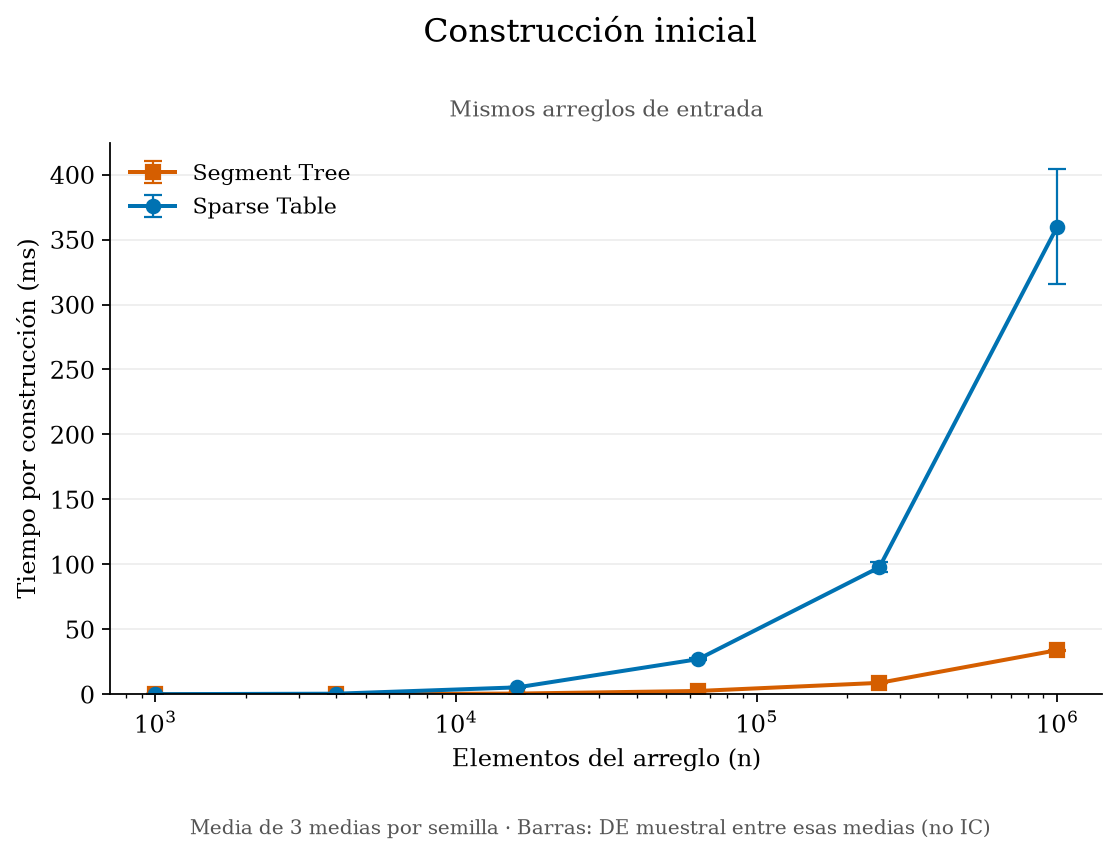
\includegraphics[width=\linewidth]{../plots/experimento_1_construccion/construction_none.png}
        \caption{Experimento 1: construcción inicial.}
        \label{fig:res-construccion}
    \end{subfigure}\hfill
    \begin{subfigure}[t]{0.49\linewidth}
        \centering
        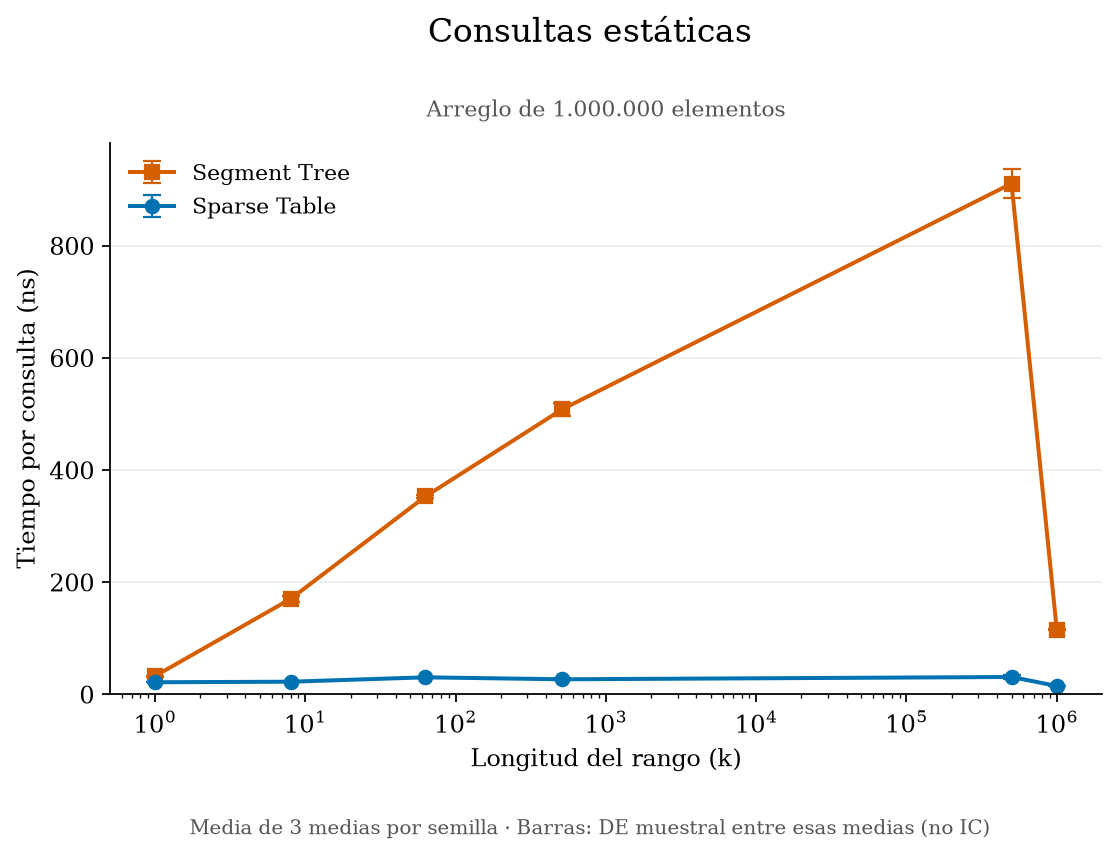
\includegraphics[width=\linewidth]{../plots/experimento_2_consultas_estaticas/static_queries_ranges_1000000.png}
        \caption{Experimento 2: consultas con \(n=10^6\).}
        \label{fig:res-consultas-estaticas}
    \end{subfigure}
    \caption{Escenario estático: costo de preparación y consultas sobre las
    estructuras ya construidas.}
    \label{fig:res-estatico}
\end{figure}

\textbf{Experimento 1.} Segment Tree presentó menor tiempo de construcción
en todos los tamaños medidos. Para \(n=10^6\), su media fue 33,953 ms,
frente a 359,880 ms de Sparse Table: una diferencia aproximada de
10,6 veces. La tendencia es consistente con las cotas \(\Theta(n)\) y
\(\Theta(n\log n)\), respectivamente, aunque estos datos no demuestran
por sí solos una complejidad asintótica.

\textbf{Experimento 2.} Sparse Table compensó parte de ese costo al consultar:
para \(n=10^6\), sus medias estuvieron entre 14,765 y 30,814 ns, frente a
32,395--910,696 ns de Segment Tree. En el rango de longitud 511, por ejemplo,
se observaron 26,714 y 507,993 ns. Este resultado se refiere a consultas
con la estructura preparada, no al costo total de una aplicación estática.
El rango completo fue más rápido que el medio en ambas estructuras;
siempre consulta el mismo intervalo \([0,n)\), por lo que no debe
interpretarse la curva como un crecimiento monótono con la longitud.

La preparación y el espacio limitan la ventaja de consultar más rápido:
con un millón de elementos, Sparse Table retuvo 305,18 MiB, frente a
30,52 MiB de Segment Tree. La tabla~\ref{tab:res-memoria} resume el espacio
sin añadir otra figura al informe.

\clearpage
\subsection{Escenario dinámico: mantenimiento y costo por ciclo}

\begin{figure}[!ht]
    \centering
    \begin{subfigure}[t]{0.49\linewidth}
        \centering
        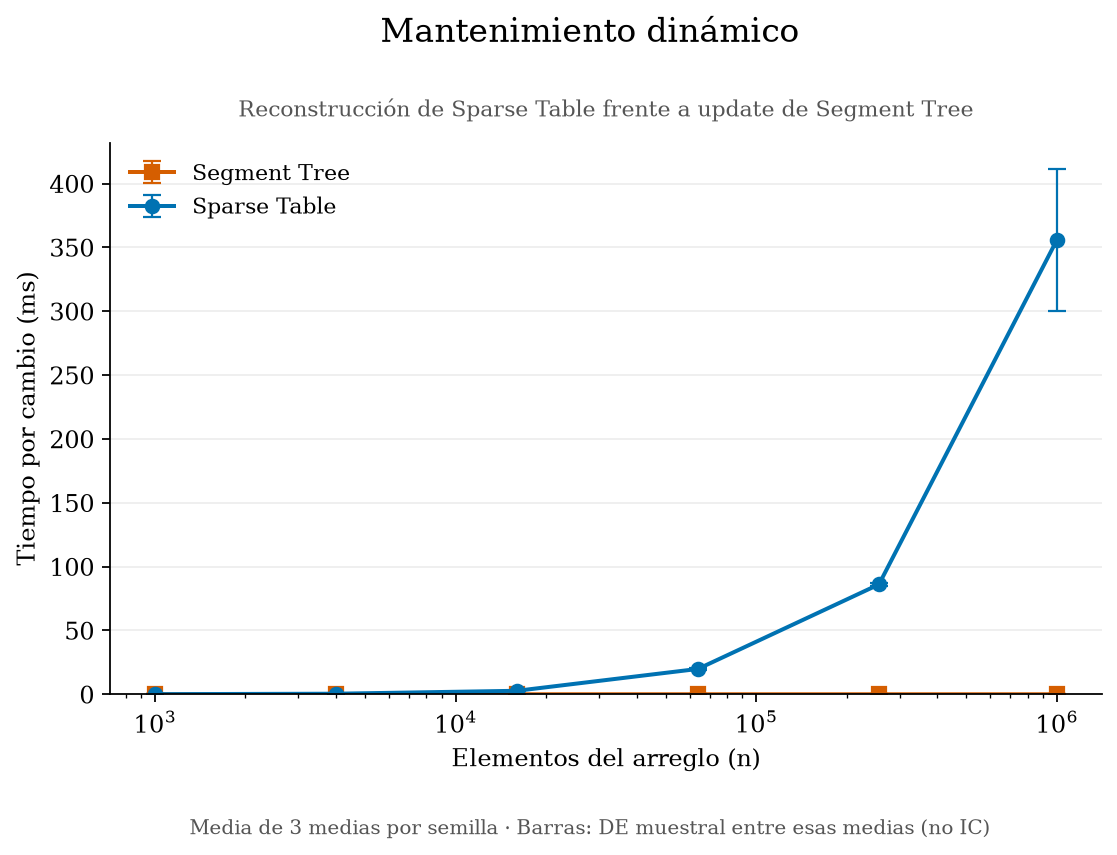
\includegraphics[width=\linewidth]{../plots/experimento_3_mantenimiento/maintenance_none.png}
        \caption{Experimento 3: reconstrucción frente a \texttt{update}.}
        \label{fig:res-mantenimiento}
    \end{subfigure}\hfill
    \begin{subfigure}[t]{0.49\linewidth}
        \centering
        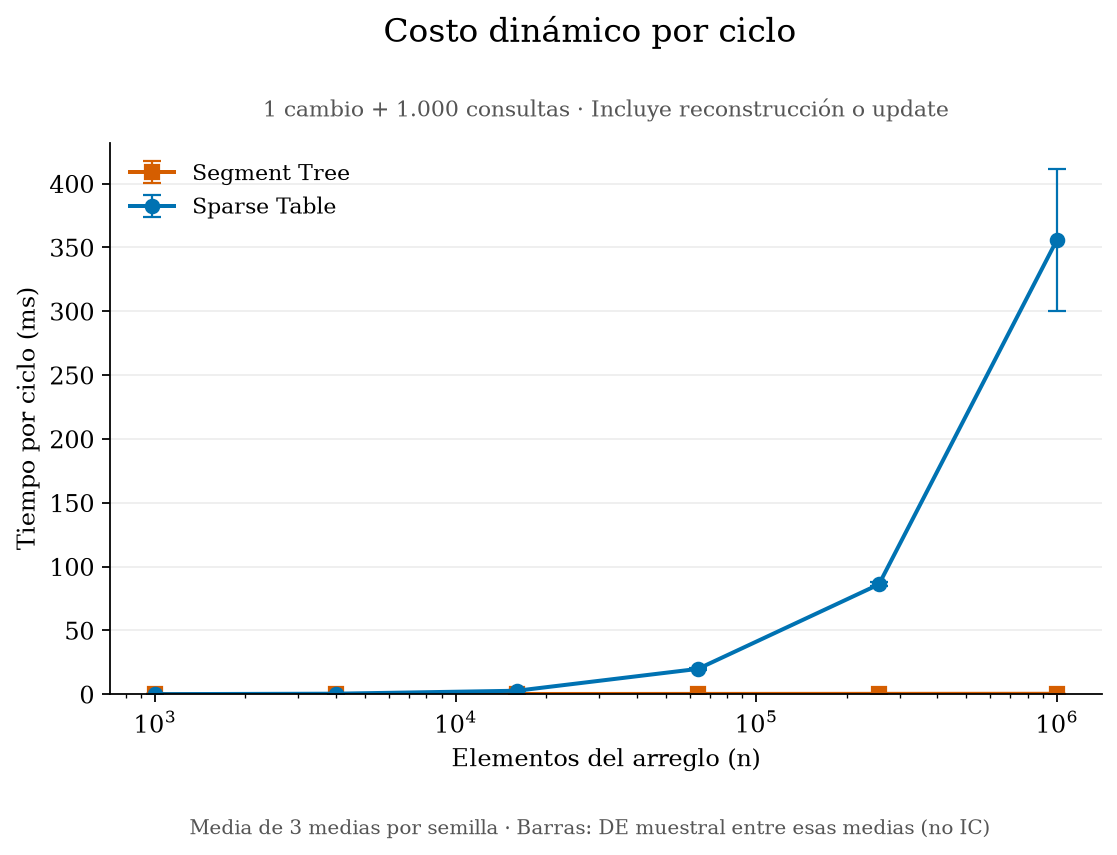
\includegraphics[width=\linewidth]{../plots/experimento_4_consultas_dinamicas/dynamic_queries_cycle.png}
        \caption{Experimento 4: un cambio y 1.000 consultas.}
        \label{fig:res-ciclo-dinamico}
    \end{subfigure}
    \caption{Escenario dinámico: mantenimiento aislado y costo combinado de
    mantenimiento y consultas del mismo ciclo.}
    \label{fig:res-dinamico}
\end{figure}

\textbf{Experimento 3.} Reconstruir Sparse Table fue más costoso que actualizar
Segment Tree en todos los tamaños. Para \(n=10^6\), las medias fueron
355,673 ms por reconstrucción y 0,831~\(\mu\)s por \texttt{update}.
Las unidades distintas de la tabla~\ref{tab:res-mantenimiento} evitan
redondear a cero las actualizaciones del árbol. Su curva casi coincide
con el eje horizontal en la figura por la diferencia de escalas,
no porque el mantenimiento sea gratuito.

\textbf{Experimento 4.} Al incluir el cambio y las 1.000 consultas de cada
ciclo, Sparse Table fue más rápida únicamente con 1.000 elementos:
0,105 ms frente a 0,156 ms. Segment Tree obtuvo menor tiempo desde
4.000 elementos entre los tamaños probados. Para \(n=10^6\), los costos
fueron 355,736 y 0,387 ms, respectivamente, unas 919 veces a favor del árbol.
El cambio de ganador se encuentra entre 1.000 y 4.000 elementos para
esta carga; no se determinó su posición exacta ni se generaliza a otra
proporción de modificaciones y consultas.

El costo por ciclo suma los intervalos de mantenimiento y consultas del
mismo método, tamaño, semilla, repetición y ciclo. La reconstrucción se
cuenta una sola vez, no por longitud de rango. Se excluyen la construcción
inicial, generación, validación, escritura y liberación: es una suma de
componentes medidos, no un cronómetro continuo de extremo a extremo.
Los diez ciclos se promedian dentro de cada repetición antes de obtener
la media por semilla; no constituyen diez repeticiones independientes.

En conjunto, las mediciones favorecen Sparse Table para consultar datos
estáticos y Segment Tree para esta carga dinámica sobre arreglos grandes.
La desviación entre semillas describe diferencias de entrada y condiciones
de ejecución que el diseño no permite separar causalmente; no se presenta
como prueba de significancia estadística.

\clearpage
% Fuentes plot_summary csv y memory_plot_summary csv de cada experimento
% Redondeo posterior a la conversion de unidades
\subsection{Resumen numérico de tiempos y memoria}

Se presentan cuatro tablas con todos los tamaños medidos. Construcción y
mantenimiento comparten las filas de \(n\), sin mezclar sus mediciones.
Los tiempos se expresan como media \(\pm\) desviación estándar muestral
entre las tres medias por semilla, con igual peso. Cada media por semilla
procede de 32 repeticiones: no es la desviación de 96 ejecuciones agrupadas
ni un intervalo de confianza. La variación dentro de cada semilla se
conserva en \texttt{summary.csv}.

\begingroup
\small
\setlength{\tabcolsep}{7pt}
\renewcommand{\arraystretch}{1.25}

\begin{table}[!ht]
    \centering
    \caption{Experimentos 1 y 3: construcción inicial y mantenimiento por cambio.}
    \label{tab:res-construccion}
    \label{tab:res-mantenimiento}
    \begin{tabular}{@{}rcccc@{}}
        \toprule
        & \multicolumn{2}{c}{Construcción inicial} & \multicolumn{2}{c}{Mantenimiento} \\
        \cmidrule(lr){2-3}\cmidrule(l){4-5}
        Elementos & Sparse Table & Segment Tree & Sparse Table & Segment Tree \\
        \(n\) & [ms] & [ms] & [ms] & [\(\mu\)s] \\
        \midrule
        1.000 & \(0{,}090 \pm 0{,}003\) & \(0{,}025 \pm 0{,}001\) & \(0{,}087 \pm 0{,}003\) & \(0{,}340 \pm 0{,}015\) \\
        4.000 & \(0{,}444 \pm 0{,}042\) & \(0{,}095 \pm 0{,}010\) & \(0{,}437 \pm 0{,}047\) & \(0{,}384 \pm 0{,}039\) \\
        16.000 & \(5{,}317 \pm 0{,}356\) & \(0{,}550 \pm 0{,}047\) & \(2{,}733 \pm 0{,}221\) & \(0{,}446 \pm 0{,}041\) \\
        64.000 & \(27{,}058 \pm 1{,}060\) & \(2{,}551 \pm 0{,}156\) & \(19{,}841 \pm 0{,}862\) & \(0{,}596 \pm 0{,}005\) \\
        256.000 & \(97{,}741 \pm 3{,}915\) & \(8{,}775 \pm 0{,}011\) & \(86{,}037 \pm 1{,}489\) & \(0{,}716 \pm 0{,}010\) \\
        1.000.000 & \(359{,}880 \pm 44{,}177\) & \(33{,}953 \pm 0{,}419\) & \(355{,}673 \pm 55{,}479\) & \(0{,}831 \pm 0{,}026\) \\
        \bottomrule
    \end{tabular}
    \par\smallskip
    \begin{minipage}{\linewidth}
        \footnotesize
        El mantenimiento compara reconstruir Sparse Table con \texttt{update}
        de Segment Tree. Solo esta última columna está en microsegundos.
    \end{minipage}
\end{table}

\begin{table}[!ht]
    \centering
    \caption{Experimento 2: tiempo por consulta estática con \(n=10^6\).}
    \label{tab:res-consultas-estaticas}
    \begin{tabular}{@{}rcc@{}}
        \toprule
        Rango & Sparse Table & Segment Tree \\
        \(k\) & [ns] & [ns] \\
        \midrule
        1 & \(21{,}436 \pm 0{,}199\) & \(32{,}395 \pm 0{,}938\) \\
        8 & \(22{,}387 \pm 0{,}752\) & \(170{,}172 \pm 5{,}207\) \\
        63 & \(30{,}239 \pm 1{,}315\) & \(352{,}761 \pm 2{,}321\) \\
        511 & \(26{,}714 \pm 1{,}720\) & \(507{,}993 \pm 11{,}615\) \\
        500.000 & \(30{,}814 \pm 3{,}387\) & \(910{,}696 \pm 26{,}032\) \\
        1.000.000 & \(14{,}765 \pm 0{,}336\) & \(114{,}839 \pm 1{,}023\) \\
        \bottomrule
    \end{tabular}
\end{table}

\begin{table}[!ht]
    \centering
    \caption{Experimento 4: tiempo por ciclo de un cambio y 1.000 consultas.}
    \label{tab:res-ciclo-dinamico}
    \begin{tabular}{@{}rcc@{}}
        \toprule
        Elementos & Sparse Table & Segment Tree \\
        \(n\) & [ms] & [ms] \\
        \midrule
        1.000 & \(0{,}105 \pm 0{,}004\) & \(0{,}156 \pm 0{,}003\) \\
        4.000 & \(0{,}457 \pm 0{,}049\) & \(0{,}182 \pm 0{,}018\) \\
        16.000 & \(2{,}772 \pm 0{,}222\) & \(0{,}218 \pm 0{,}015\) \\
        64.000 & \(19{,}889 \pm 0{,}864\) & \(0{,}284 \pm 0{,}005\) \\
        256.000 & \(86{,}090 \pm 1{,}488\) & \(0{,}332 \pm 0{,}007\) \\
        1.000.000 & \(355{,}736 \pm 55{,}485\) & \(0{,}387 \pm 0{,}003\) \\
        \bottomrule
    \end{tabular}
\end{table}

\begin{table}[!ht]
    \centering
    \caption{Memoria retenida y pico total durante el mantenimiento.}
    \label{tab:res-memoria}
    \begin{tabular}{@{}rrrrr@{}}
        \toprule
        & \multicolumn{2}{c}{Sparse Table} & \multicolumn{2}{c}{Segment Tree} \\
        \cmidrule(lr){2-3}\cmidrule(l){4-5}
        Elementos & Retenida & Pico total & Retenida & Pico total \\
        \(n\) & [MiB] & [MiB] & [MiB] & [MiB] \\
        \midrule
        1.000 & 0{,}15 & 0{,}32 & 0{,}03 & 0{,}03 \\
        4.000 & 0{,}73 & 1{,}53 & 0{,}12 & 0{,}12 \\
        16.000 & 3{,}42 & 7{,}08 & 0{,}49 & 0{,}49 \\
        64.000 & 15{,}63 & 32{,}23 & 1{,}95 & 1{,}95 \\
        256.000 & 70{,}31 & 144{,}53 & 7{,}81 & 7{,}81 \\
        1.000.000 & 305{,}18 & 625{,}61 & 30{,}52 & 30{,}52 \\
        \bottomrule
    \end{tabular}
\end{table}

\endgroup

\endgroup
